\documentclass[a4paper]{article}

\usepackage[a4paper,margin=1.5cm]{geometry}
\usepackage[utf8]{inputenc}
\usepackage{amsmath,amsfonts,stmaryrd,amssymb}
\usepackage[francais]{babel}
\usepackage{fancyvrb}
\usepackage{graphicx}
\usepackage{subcaption}
\usepackage{enumerate}
\usepackage{todonotes}
\usepackage[ruled]{algorithm2e}
\usepackage[pdftex,hidelinks]{hyperref}
\usepackage{placeins}
\usepackage{fontawesome}

\usepackage[framemethod=tikz]{mdframed}
%\usetikzlibrary{calc}

\title{Etudier la qualité numérique d'un code avec Verrou}
\author{Bruno Lathuilière\\
  \tt \{bruno.lathuiliere\}@edf.fr
}
\date{Mise à jour \cite{tpVerrou} pour verrou v2.7.0 (à venir)}

\newcommand{\note}[1]{\todo{%
    \protect\rotatebox{90}{% 
      \protect\begin{minipage}{13em}%
        \footnotesize #1%
      \protect\end{minipage}}}}

\def\mdcmdlinespacing{\hspace{-2.5em}}
\mdfdefinestyle{commandline}{
  leftmargin=10pt,
  rightmargin=10pt,
  innerleftmargin=15pt,
  middlelinecolor=black!50!white,
  middlelinewidth=2pt,
  frametitlerule=false,
  backgroundcolor=black!5!white,
  frametitle={Command line},
  frametitlefont={\normalfont\sffamily\color{white}\mdcmdlinespacing},
  frametitlebackgroundcolor=black!50!white,
  nobreak,
}
\newenvironment{commandline}{
  \begin{mdframed}[style=commandline]
}{
  \end{mdframed}
}


\def\mdfilename{File}
\mdfdefinestyle{file}{
  innertopmargin=1.6\baselineskip,
  innerbottommargin=0.8\baselineskip,
  topline=false, bottomline=false,
  leftline=false, rightline=false,
  leftmargin=2cm,
  rightmargin=2cm,
  singleextra={%
    \draw[fill=black!10!white](P)++(0,-1.2em)rectangle(P-|O);
    \node[anchor=north west]
    at(P-|O){\ttfamily\mdfilename};
    %
    \def\l{3em}
    \draw(O-|P)++(-\l,0)--++(\l,\l)--(P)--(P-|O)--(O)--cycle;
    \draw(O-|P)++(-\l,0)--++(0,\l)--++(\l,0);
  },
  nobreak,
}
\newenvironment{file}[1][Fichier]{
  \def\mdfilename{#1}
  \begin{mdframed}[style=file]
}{
  \end{mdframed}
}

\mdfdefinestyle{question}{
  innertopmargin=1.2\baselineskip,
  innerbottommargin=0.8\baselineskip,
  roundcorner=5pt,
  nobreak,
  singleextra={%
    \draw(P-|O)node[xshift=1em,anchor=west,fill=white,draw,rounded corners=5pt]{%
      Question \theQuestion\questionTitle};
  },
}
\newcounter{Question}
\newenvironment{question}[1][\unskip]{
  \bigskip
  \stepcounter{Question}
  \def\questionTitle{ #1}
  \begin{mdframed}[style=question]
  }{
  \end{mdframed}
}

\mdfdefinestyle{warning}{%
  topline=false, bottomline=false,
  leftline=false, rightline=false,
  nobreak,
  singleextra={%
    \draw(P-|O)++(-0.5em,0)node(tmp1){};
    \draw(P-|O)++(0.5em,0)node(tmp2){};
    \fill[black,rotate around={45:(P-|O)}](tmp1)rectangle(tmp2);
    \node at(P-|O){\color{white}\scriptsize\bf !};
    \draw[very thick](P-|O)++(0,-1em)--(O);%--(O-|P);
  }
}
\newenvironment{warn}[1][Attention :]{
  \begin{mdframed}[style=warning]
    \noindent{\bf #1}
}{
  \end{mdframed}
}


\mdfdefinestyle{info}{%
  topline=false, bottomline=false,
  leftline=false, rightline=false,
  nobreak,
  singleextra={%
    \fill[black](P-|O)circle[radius=0.4em];
    \node at(P-|O){\color{white}\scriptsize\bf i};
    \draw[very thick](P-|O)++(0,-0.8em)--(O);%--(O-|P);
  }
}
\newenvironment{info}[1][NB :]{
  \begin{mdframed}[style=info]
    \noindent{\bf #1}
}{
  \end{mdframed}
}



% TikZ file tree
\def\FTdir(#1,#2,#3){%
  \FTfile(#1,{{\color{black!40!white}\faFolderOpen}\hspace{0.2em}#3})
  (tmp.west)++(0.8em,-0.4em)node(#2){}
  (tmp.west)++(1.5em,0)
  ++(0,-1.3em) 
}
\def\FTfile(#1,#2){%
  node(tmp){}
  (#1|-tmp)++(0.6em,0)
  node(tmp)[anchor=west,black]{\tt #2}
  (#1)|-(tmp.west)
  ++(0,-1.2em) 
}
\def\FTroot{tmp.west}



\begin{document}
\maketitle


\section*{Contexte et objectifs}

Dans ce TP, nous nous intéressons à l'étude de la qualité numérique d'un code
réalisant le calcul approché de l'intégrale d'une fonction $f$ sur un intervalle
$[a, b]$ :
\begin{align*}
  I &= \int_{a}^{b} f(x) \; \text{d}x.
\end{align*}

Numériquement, ce calcul est réalisé à l'aide de la méthode des rectangles. Si
$n$ est le nombre de rectangles, on a :
\begin{align*}
  I_n &= \sum_{i=1}^n f(x_i) \; h,
\end{align*}
où l'on a noté $h = \frac{b - a}{n}$ la largeur des rectangles d'intégration, et
si on partitionne $[a, b]$ en $n$~sous-intervalles de longueur~$h$, on note
$x_i = a + (i-\frac{1}{2}) \, h$ le point central du $i$-ème sous-intervalle.

\bigskip

On a mathématiquement les résultats de convergence suivants (dans $\mathbb{R}$) :
\begin{align*}
  I_n \xrightarrow[n \to \infty]{} I,
\end{align*}
avec une vitesse de convergence au premier ordre :
\begin{align*}
  \varepsilon_n := \left\vert I_n - I \right\vert = \mathcal{O}\left(\frac{1}{n}\right).
\end{align*}
C'est cette dernière propriété qui est utilisée ici pour effectuer une vérification
du code : si on considère le cas $f = \cos$, $a = 0$ et $b = 1$, on connaît
la valeur exacte $I=1$. Un tracé de $\varepsilon_n$ en fonction de $n$ en
échelle logarithmique nous permettra donc de vérifier la vitesse de convergence.

\bigskip

\begin{info}[Remarque :]
  du point point de vue de la vérification numérique, il est intéressant de
  remarquer que ce problème est entièrement décrit par des données~($a$, $b$)
  représentables en format flottant, que le résultat exact~($I$) est lui-même
  représentable, mais que le calcul fera intervenir des nombres non
  nécessairement re\-pré\-sen\-tables~\mbox{($h$, $x_i$)} voire
  irrationnels~($\cos(x_i)$).
\end{info}

\bigskip

Sur la base de ce cas-test de vérification, nous allons mener l'étude de la
qualité numérique du code de calcul de l'intégrale à l'aide de l'outil
Verrou~\cite{verrou, verrou-hpc}. Bien que le code étudié soit ici petit et facilement
manipulable, toutes les techniques présentées ici peuvent passer à l'échelle
pour de grands codes industriels (au prix parfois d'un peu d'outillage
informatique permettant d'automatiser certaines tâches). Une étude a par exemple
été réalisée en suivant la même méthodologie d'analyse pour le code de calcul
mécanique code\_aster~\cite{fevotte2017}.

\subsection*{Prérequis}

La réalisation de ce TP nécessite des connaissances (au moins) élémentaires en
Python, C++ (avec le compilateur Gnu) et Gnuplot.

\medskip

Par ailleurs, nous supposons dans ce document que Verrou (version
$\geqslant 2.7.0$) a été correctement installé. Si ce n'est pas le cas, merci de
vous reporter aux instructions disponibles sur la page GitHub du projet :
\begin{center}
  \url{https://github.com/edf-hpc/verrou/tree/v2.7.0}
\end{center}

La documentation de réference de la dernière version stable \url{https://edf-hpc.github.io/verrou/vr-manual.html}
vous sera utile. Si vous préférez utiliser la version master de verrou, pensez à générer la documentation (cf. procédure d'installation).



\subsection*{Code source fourni}

Nous décrivons ici l'organisation générale du code source servant de base à la
réalisation de ce TP. L'organisation générale des fichiers est indiquée sur la
figure~\ref{fig:src} :
\begin{description}
\item[\tt work]: répertoire dans lequel le TP se déroule. Il contient notamment
  les fichiers suivants (les autres fichiers ne sont pas utiles dans un premier
  temps, et seront décrits par la suite) :
  \begin{description}
  \item[\tt integrate.hxx]: le code source C++ réalisant le calcul d'intégrale
    proprement dit.
  \item[\tt unitTest.cxx]: le code source C++ réalisant l'étude de convergence
    permettant de le vérifier. La convergence est testée en réalisant le calcul
    d'intégrale pour différents nombres de rectangles $n$ variant selon une
    suite géométrique entre 1 et 100~000. La raison de cette suite géométrique
    est passée comme argument en ligne de commande du binaire généré
    (\texttt{unitTest}). Pour chaque calcul d'intégrale pour un nombre de
    rectangles donné, les résultats sont affichés sur 3 colonnes : $n$, $I_n$
    et~$\varepsilon_n$. Un exemple d'utilisation du programme est donné sur la
    figure~\ref{fig:integrate.cl}.
  \item[\tt cvPlot]: un \textit{shell}-script permettant de lancer l'étude de
    convergence et de générer le graphe correspondant (à l'aide du script
    gnuplot \texttt{cvPlot.gp}). Un exemple de graphe produit est illustré en
    figure~\ref{fig:cvplot_10}.
  \item[\tt Makefile]: permet d'orchestrer la compilation du code étudié,
    ainsi que l'étude de convergence correspondant à sa vérification. 
  \item[\tt util]: contient des scripts utilitaires, qui pourront éventuellement
    être ré-utilisés dans un contexte autre que celui de ce TP.
  \end{description}
\item[\tt corrige]: contient des sous-répertoires correspondant à certaines
  étapes clés du processus (correspondant aux sections du présent document). En
  cas de doute ou de blocage durant la réalisation du TP, il est toujours
  possible de se référer au corrigé de l'étape en cours afin d'avoir un aperçu
  de la solution. La structure de chaque sous-répertoire \texttt{etapeX.Y} est
  similaire à celle de \texttt{work}. Le \texttt{Makefile} fourni permet de
  réaliser tout ce qui est nécessaire à l'étape correspondante.
%% \item[\tt libeft]: contient les sources de la bibliothèque \texttt{libEFT}, qui
%%   pourra servir à implémenter les algorithmes compensés dans la
%%   partie~\ref{sec:fix.sum} du TP. La documentation de l'API fournie par cette
%%   bibliothèque est disponible dans le fichier \texttt{README.pdf}.
\end{description}

\begin{figure}[htb]
  \begin{subfigure}[b]{0.4\linewidth}
    \centering
\begin{tikzpicture}%
  \draw[color=black!60!white]
  \FTdir(\FTroot,top,tp-verrou){
    \FTdir(top,work,work){
      \FTfile(work,integrate.hxx)
      \FTfile(work,unitTest.cxx)
      \FTfile(work,cvPlot)
      \FTfile(work,cvPlot.gp)
      \FTfile(work,Makefile)
      \FTdir(work,util,util)}
    ++(0,-0.5em)
    \FTdir(top,corrige,corrige) {
      \FTdir(corrige,x,etape1.0)
      \FTdir(corrige,x,etape1.1)
      \FTdir(corrige,x,etape2.0)
      \FTfile(corrige,...)}
    ++(0,-0.5em)
%    \FTdir(top,libeft,libeft){
%      \FTfile(libeft,README.pdf)
%    }
  };
  \end{tikzpicture}
    \caption{Organisation générale du code source de ce TP}
    \label{fig:src}
  \end{subfigure}
  \begin{subfigure}[b]{0.62\linewidth}
    \def\mdcmdlinespacing{\hspace{-1em}}
    \begin{commandline}
\begin{verbatim}
$ ./unitTest 10

         1 1.1107207345395915 1.1072073453959153e-01
        10 1.0010288241427083 1.0288241427083289e-03
       100 1.0000102809119049 1.0280911904914092e-05
      1000 1.0000001028083909 1.0280839091159066e-07
     10000 1.0000000010279895 1.0279894713249860e-09
    100000 1.0000000000099656 9.9655839136403301e-12
\end{verbatim}
    \end{commandline}
    \caption{Exemple d'utilisation du programme}
    \label{fig:integrate.cl}
  \end{subfigure}
  \caption{Code source fourni}
\end{figure}

\begin{figure}[htb]
  \centering
  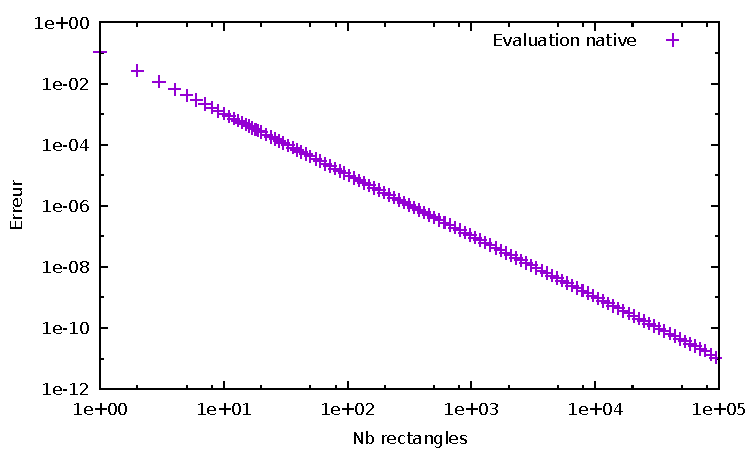
\includegraphics[width=0.75\textwidth]{cvPlot_10.pdf}
  \caption{Convergence du calcul d'intégrale}
  \label{fig:cvplot_10}
\end{figure}

\newpage

\section{Analyse du code en double précision}

Le code tel qu'il est fourni dans sa version de base utilise le calcul en double
précision. Nous nous proposons dans un premier temps de réaliser l'analyse de ce
code, avant de passer dans une deuxième partie à l'analyse (un peu plus
délicate) d'une version en simple précision.

\begin{question}
  Familiarisez-vous avec le code fourni.
  \begin{enumerate}[(a)]
  \item Étudiez le code source des fonctions \texttt{integrate} (dans le
    fichier \texttt{integrate.hxx}) et \texttt{testConvergence} (dans le fichier
    \texttt{unitTest.cxx}).
  \item Étudiez le \texttt{Makefile} fourni. Compilez le programme
    \texttt{unitTest} et lancez-le manuellement.
  \item Lancez le script \texttt{cvPlot} et étudiez la courbe de convergence
    produite dans \texttt{cvPlot.pdf} (vous devriez obtenir une courbe similaire
    à celle de la figure~\ref{fig:cvplot_10}). Est-elle satisfaisante ?
  \end{enumerate}
\end{question}

\bigskip

Avant de commencer à utiliser Verrou pour analyser un code, il est préférable de
vérifier que les perturbations liées à l'environnement Valgrind lui-même ne sont
pas déjà de nature à perturber l'exécution.

\begin{question}
  Vérifiez la reproductibilité des résultats fournis par code, dans tous les cas
  suivants :\\
  \begin{tabular}{ll}
    --- Mode natif :          & \tt ./unitTest\\
    --- Valgrind sans outil : & \tt valgrind --tool=none ./unitTest\\
    --- Valgrind/memcheck :   & \tt valgrind ./unitTest\\
    --- Verrou sans perturbation : & \tt valgrind --tool=verrou
                                     --rounding-mode=nearest ./unitTest
  \end{tabular}
\end{question}

\subsection{Evaluation des erreurs de calcul avec Verrou}

On se propose ici d'évaluer la part des erreurs de calcul dans l'erreur globale,
en perturbant l'étude de convergence avec les arrondis aléatoires de Verrou.

\begin{question}
  \begin{enumerate}[(a)]
  \item Familiarisez-vous avec Verrou. Par exemple, lancez Verrou sur
    l'interpréteur Python :

    \qquad{\ttfamily valgrind --tool=verrou --rounding-mode=random python3}
  
    et essayez de réaliser quelques opérations flottantes plusieurs fois.

  \item Expliquez ce qu'il se passe dans chacun des cas suivants (vous devriez
    obtenir des résultats similaires à ceux présentés ci-dessous) :
    \begin{enumerate}[(i)]
    \item {\tt sum((0.1*i for i in range(100)))}
    \item {\tt sum((0.125*i for i in range(100)))}
    \item {\tt from math import cos; cos(42.)}
    \end{enumerate}
  \end{enumerate}
\end{question}
\begin{commandline}
\begin{verbatim}
$ valgrind --tool=verrou --rounding-mode=random python3

>>> # cas (i)
>>> sum((0.1*i for i in range(100)))
495.00000000000034
>>> sum((0.1*i for i in range(100)))
494.99999999999983

>>> # cas (ii)
>>> sum((0.125*i for i in range(100)))
618.75
>>> sum((0.125*i for i in range(100)))
618.75


>>> # cas (iii)
>>> from math import cos
>>> cos(42.)
-0.39998531498835127
>>> cos(42.)
-0.39998531498835127
\end{verbatim}
\end{commandline}
Pour plus de détails sur la bibliothèque mathématique, voir partie \ref{ref:libm} page \pageref{ref:libm}.

\bigskip

\begin{question}
  Utilisation de verrou sur \texttt{unitTest} en mode exploratoire.
  \begin{enumerate}[(a)]
  \item Faites tourner le \texttt{unitTest} en mode natif et stocker le résultat
    dans un fichier.
  \item Faites tourner le \texttt{unitTest} avec verrou en mode random plusieurs
    fois et stocker les résultats dans des fichiers séparés.
  \item Comparer les résultats avec meld (ou un autre comparateur
    graphique). La séquence de commande doit ressembler à celle
    affichée ci-dessous.
  \item Quelles sont les limitations de cette approche?
  \end{enumerate}
\end{question}

\begin{commandline}
\begin{verbatim}
$ ./unitTest > out.ref 
$ valgrind --tool=verrou --rounding-mode=random ./unitTest > out.random_1
$ valgrind --tool=verrou --rounding-mode=random ./unitTest > out.random_2
$ valgrind --tool=verrou --rounding-mode=random ./unitTest > out.random_3
$ meld out.ref out.random_1
$ meld out.ref out.random_2
$ meld out.ref out.random_3
\end{verbatim}
\end{commandline}


Pour faire face à ces limitations, nous allons calculer pour chaque
point de convergence l'estimateur d'erreur flottante calculer par verrou. 
Le script \texttt{util/csv-estimator} fourni avec ce TP permet de les
calculer à partir de plusieurs
résultats, formattés comme des fichiers textes en colonnes séparées par des
espaces. Le script prend en argument une liste de fichiers contenant les
résultats à analyser, et affiche sur sa sortie standard les résultats du premier fichier au même
format mais en ajoutant des colonnes supplémentaires avec les options \texttt{--col-rel} ou \texttt{--col-abs} dans la
ligne de commande. Ces nouvelles colonnes correspondent à l'estimateur relatif (respectivement absolu) de Bernouilli.

Autrement dit, si le fichier numéro $k$ contient la donnée $x_{i,j}^k$ dans sa
$i$-ème ligne et $j$-ème colonne, la sortie contiendra à la même place la valeur
$x_{i,j}^1$.

En listant des colonnes supplémentaires avec l'option
\texttt{--col-rel=INDEX} (respectivement \texttt{--col-abs=INDEX}) dans la
ligne de commande, on ajoute à la sortie une colonne supplémentaire
contenant pour chaque ligne $i$ :
\begin{equation*}
  \hat{s}^{\text{rel}}_{i} = \frac{\max_k ( \left|x_{i,j}^k
    -x_{i,j}^1\right|) }{\left| x_{i,j}^1 \right|}, \qquad \forall i
  \quad with \quad j=INDEX
\end{equation*}

\begin{equation*}
  \hat{s}^{\text{abs}}_{i} = \max_k ( \left|x_{i,j}^k
  -x_{i,j}^1\right| ) , \qquad \forall i   \quad with \quad j=INDEX.
\end{equation*}


Enfin, les estimateurs maximaux (absolu et relatif) sont  imprimés sur la sortie d'erreur. S'il
dépasse le critère maximum donné par l'utilisateur à l'aide de l'option
\texttt{--est-max}, le script renvoie une erreur (code de retour: 1).

\bigskip

Dans notre cas, on pourrait par exemple obtenir les sorties suivantes:
\begin{commandline}
\begin{verbatim}
$ ./util/csv-estimator --col-abs=2 --est-max=1e-15 cvPlot.dat cvPlot?*.dat
\end{verbatim}
{\footnotesize
\begin{verbatim}
    # (1)                      # (2)                   # (3)                      # (4)                   
    # input col 1 (first)      # input col 2 (first)   # input col 2 (est abs)    # input col 3 (first)     
    1.00000000000000000e+00    1.11072073453959153e+00 7.79696801233676114e-17    1.10720734539591581e-01 
    1.00000000000000000e+01    1.00102882414270855e+00 1.49845834987280771e-16    1.02882414270843991e-03 
    1.00000000000000000e+02    1.00001028091190602e+00 6.97757113268229776e-16    1.02809119060243148e-05 
    1.00000000000000000e+03    1.00000010280839802e+00 4.07829579359800326e-15    1.02808397961506870e-07 
    1.00000000000000000e+04    1.00000000102823439e+00 1.41491103815151729e-13    1.02823444203536951e-09 
    1.00000000000000000e+05    1.00000000000957856e+00 2.23909591127846818e-13    9.57850465610476931e-12 
    max abs estimator: 2.10476081008437177e-12
\end{verbatim}
}
\begin{verbatim}
$ echo $?
    1
\end{verbatim}
\end{commandline}
\noindent dans lesquelles les 4 colonnes représentent:
\begin{enumerate}
\item le nombres de rectangles (normalement identiques entre exécutions),
\item les résultats obtenus en natif,
\item {\bf l'erreur flottante estimé par verrou} (c'est cette colonne qui
  nous intéresse),
\item l'erreur de méthode pour l'exécution native.
\end{enumerate}

\bigskip

\begin{warn}
  Une erreur classique à éviter est la comparaison de résultats sortis par le
  code avec trop peu de chiffres significatifs.
\end{warn}

\begin{question}
  \begin{enumerate}[(a)]
  \item Modifiez les scripts \texttt{cvPlot} et \texttt{cvPlot.gp} pour analyser
    3~exécutions de l'étude de convergence perturbées avec Verrou, et en déduire
    une évaluation de l'erreur de calcul. (Si vous n'êtes pas familier avec la
    syntaxe \texttt{gnuplot}, la commande modifiée pour tracer deux courbes est
    affichée ci-dessous.) On devrait obtenir une courbe similaire à celle
    présentée sur la figure~\ref{fig:cvplot_11}.

  %% \item Que se passe-t-il selon qu'on intègre les résultats IEEE (non perturbés)
  %%   ou pas à la statistique ?

  %% \item (optionnelle) Que se passe-t-il avec des statistiques sur
  %%   10~échantillons~? Quel est l'impact du mode ``proportionnel'' de verrou ?
  %%   Rappel : on active ce mode d'arrondi à l'aide de l'option :\\
  %%   \strut\qquad{\tt --rounding-mode=average}
  %% \item (optionnelle [plus simple après le delta-debugging]) Comparer les différents mode d'arrondis en tracant les histogrammes à l'aide de la commande \texttt{verrou\_plot\_stat}.
  \end{enumerate}
\end{question}

\begin{file}[cvPlot.gp]
\begin{verbatim}
  ...
  plot "cvPlot.dat"  using 1:3 title "Evaluation native", \
       "cvPlot.stat" using 1:3 title "Estimation verrou"
  ...
\end{verbatim}
\end{file}

\bigskip

A l'issue de cette étape, l'analyse Verrou devrait permettre d'obtenir des
résultats similaires à ceux de la figure~\ref{fig:cvplot_11}. Ceci permet de
confirmer la première impression : les erreurs de calcul sont assez négligeables
dans cette gamme d'utilisation du code.

\begin{figure}[htbp]
  \centering
  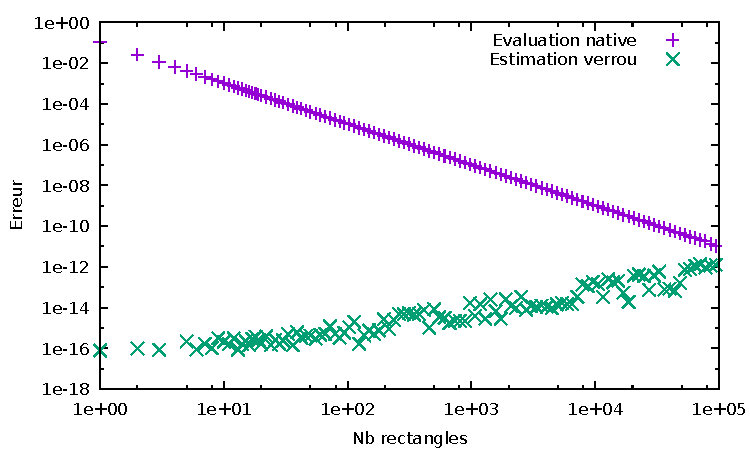
\includegraphics[width=0.75\textwidth]{cvPlot_11.pdf}
  \caption{Convergence du calcul d'intégrale et évaluation de l'erreur de calcul
  avec Verrou}
  \label{fig:cvplot_11}
\end{figure}

\begin{warn}
  Ce TP fournit le script ./util/csv-estimator pour être capable de visualiser
  l'estimateur d'erreur pour un ensemble de points. Ce script dépend du format
  utilisé par le programme (ici csv). On est parfois amené à écrire des scripts
  équivalents pour s'adapter à un code industriel. Lorsque qu'on s'intéresse à
  des variables simples, on peut utiliser directement l'outil
  \texttt{verrou\_plot\_stat} distribué avec verrou. Ce TP aborde cet outil
  dans la partie \ref{ref:plotStat} (page \pageref{ref:plotStat}).
  
\end{warn}



\section{Analyse du code en simple précision}
\label{ref:AnalyseSimple}

Nous nous proposons maintenant d'utiliser une arithmétique en simple précision
dans notre calcul d'intégration.

\begin{question}
  \begin{enumerate}[(a)]
  \item Modifiez \texttt{integrate.hxx} pour basculer en calcul en simple
    précision.
  \item Relancez l'analyse précédente et interprétez les résultats.
  \end{enumerate}
\end{question}





\subsection{Déboguage numérique à l'aide du \textit{Delta-Debugging}}

Nous nous proposons maintenant de rechercher les instabilités à l'aide
d'une approche par bisection, en sélectionnant les portions de code perturbées
par Verrou. C'est ce que permet de faire les outils \texttt{verrou\_dd\_sym} et \texttt{verrou\_dd\_line}, livrés avec
Verrou. \texttt{verrou\_dd\_line}, (respectivement \texttt{verrou\_dd\_sym}) s'utilise de la manière suivante :
\begin{center}
  \tt verrou\_dd\_line ./DD\_RUN ./DD\_CMP
\end{center}

Dans la commande ci-dessus, les deux arguments sont des commandes, qui doivent
automatiser respectivement le lancement du code avec Verrou, et la comparaison
d'un résultat à une référence. Ces deux commandes doivent respecter les
prototypes suivants: \medskip
\begin{itemize}
\item[\tt DD\_RUN DIR]\strut\\
  Lance le code à analyser dans Verrou, et range les résultats dans le
  répertoire \texttt{DIR}. Un exemple classique de script de lancement pourrait
  ressembler à :

\begin{file}[ddRun]
\begin{verbatim}
#!/bin/bash

# Récupération des arguments
DIR=$1

# Lancement du code dans Verrou
valgrind --tool=verrou --rounding-mode=random ...

# Rangement des résultats dans le répertoire cible
cp  ...  ${DIR}/...

# Si possible on préfére configurer le code pour écrire
# directement dans le répertoire ${DIR} (pour être réentrant)

\end{verbatim}
\end{file}

  \medskip
\item[\tt DD\_CMP REFDIR CURDIR]\strut\\
  Effectue la vérification des résultats contenus dans le répertoire
  \texttt{CURDIR}, potentiellement en les comparant à des résultats ``de
  référence'' rangés dans \texttt{REFDIR}. Ces résultats ``de référence''
  correspondent à une exécution du code (tel que lancé par \texttt{DD\_RUN}) non
  perturbé par Verrou. \texttt{DD\_CMP} renvoie 0 si et seulement si le résultat
  contenu dans \texttt{CURDIR} est considéré comme valide.

  Une trame pour le script de validation pourrait être donnée par:
\begin{file}[ddCmp]
\begin{verbatim}
#!/bin/bash

# Récupération des arguments
REFDIR=$1
CURDIR=$2

# Validation des résultats contenus dans ${CURDIR}
# (éventuellement par comparaison à ceux de ${REFDIR})
...
\end{verbatim}
\end{file}
ou bien par un script python :
\begin{file}[ddCmp.py]
\begin{verbatim}
#!/usr/bin/python3
import sys
import os
def extractValue(rep):
    USER_DEFINED_CODE_TO_PARSE_RESULT

if __name__=="__main__":
    if len(sys.argv)==2:
        #this case is to be compatible with the extract script
        # of verrou_plot_stat and to simplify debug
        print(extractValue(sys.argv[1]))
    if len(sys.argv)==3:
        valueRef=extractValue(sys.argv[1])
        value=extractValue(sys.argv[2])
        relDiff=abs((value-valueRef)/valueRef)

        if relDiff < USER_DEFINED_TOLERANCE:
            sys.exit(0) #OK
        else:
            sys.exit(1) #KO
\end{verbatim}
\end{file}

\end{itemize}

\begin{info}
  la mise au point de ces deux scripts est l'unique action à réaliser afin
  d'étudier un code avec les fonctionnalités de \textit{Delta-Debugging} de
  Verrou. Il est donc important de bien comprendre le comportement attendu de
  ces scripts, afin de pouvoir les adapter au cas d'intérêt dans un contexte
  plus complexe que celui de ce TP.
\end{info}

\bigskip

À chaque fois que \texttt{verrou\_dd\_line} cherche à tester une combinaison de
fonctions/lignes perturbées, le code est lancé à l'aide de \texttt{DD\_RUN}, et
ses résultats sont analysés à l'aide de \texttt{DD\_CMP}. Si un échec signifie
que la configuration est instable, un succès ne suffit pas pour prouver qu'elle
est stable (on pourrait avoir eu de la chance dans les tirages aléatoires). Pour
cette raison, une configuration n'est considérée comme stable qu'après un
certain nombre d'exécutions validées. Ce nombre est porté à 5 par défaut, mais
peut être réglé à l'aide de l'option \texttt{--nruns=}.

\bigskip

Durant son exécution, \texttt{verrou\_dd\_line} réalise de nombreux essais, et les
résultats correspondants sont rangés dans une arborescence similaire à celle
décrite en figure~\ref{fig:dd}, et dont la description détaillée est donnée en
annexe~\ref{app:dd}. Dans un premier temps, pour interpréter les résultats du
\textit{Delta-Debugging}, il suffit de savoir que les utilitaires
\texttt{verrou\_dd\_line} (respectivement \texttt{verrou\_dd\_sym})créent dans
le répertoire \texttt{dd.line} (respectivement \texttt{dd.sym}) des liens symboliques pour
chaque configuration 1-minimal. Pour savoir à quelle ensemble de ligne ou de
symboles, correspond à cette configuration il suffit de regarder le fichier d'inclusion et
d'exclusion qui s'y trouve.

Pour les codes C++ les noms de symbole n'étant pas facile à lire
il peut être nécessaire d'utiliser la commande \texttt{c++filt}. Dans la pratique,
on utilise rarement cette commande, 
le résumé founit par les algorithmes de type rddmin, sur la sortie standard
en fin d'execution ou dans le fichier \texttt{dd.line/rddmin\_summary} font ce travail pour vous.

\bigskip

\begin{warn}
  les fichiers contenus dans les répertoires \texttt{dd.line} \texttt{dd.sym}
  servent à contenir les résultats mais aussi de cache pour éviter de refaire plusieurs fois les mêmes essais. Il
  est donc nécessaire de supprimer ces répertoires avant une exécution du
  \textit{delta-debugging} afin d'éviter que l'analyse soit perturbée par des
  scories d'analyses précédentes ou d'utiliser l'option \texttt{--cache} pour dire comment ré-utiliser ce cache.
\end{warn}

\begin{question} Réalisez le \textit{delta-debugging} du code de calcul
  d'intégrale :
  \begin{enumerate}[(a)]
  \item Mettez au point le script \texttt{DD\_RUN}, permettant d'automatiser le
    lancement de \texttt{unitTest} avec Verrou, et la sauvegarde de ses
    résultats dans un fichier de votre choix dans le répertoire indiqué en
    argument.
  \item Dans le langage de votre choix (python ou bash via csv-estimator),
    mettez au point le script \texttt{DD\_CMP}, permettant de comparer les
    résultats de \texttt{unitTest}, en cohérence avec le stockage mis en place
    dans \texttt{DD\_RUN}. L'analyse de la courbe de convergence pourra permettre
    de dimensionner de manière adéquate le seuil de tolérance dans la validation
    des résultats.
  \item Testez vos deux scripts.
  \item Lancez \texttt{verrou\_dd\_line} et analysez les résultats. Vous devriez
    trouver deux lignes instables.
  \item (optionnel) Étudiez l'impact des deux paramètres-clés de la recherche :
    \begin{itemize}
    \item le seuil de tolérance utilisé par \texttt{DD\_CMP},
    \item le nombre d'exécutions requis pour valider une configuration, fixé par
       l'option \texttt{--nruns=}.
    \end{itemize}
  \item (optionnel) Étudiez l'impact des options de compilation (avec ou sans -g).
  \item Pourquoi est-ce une mauvaise idée d'utiliser \texttt{diff} pour le script
    \texttt{DD\_CMP} dans ce cas?
  \end{enumerate}
\end{question}

\subsection{Détection des branchements instables grâce à \texttt{post\_verrou\_dd}}
Le delta-debug permet de détecter l'origine des erreurs dans le code
source, mais parfois la correction ne doit pas se faire au niveau de
l'origine, mais là où elles sont amplifiées.
Un changement du flot d'exécution du code,
lorsqu'un branchement dépend d'une valeur perturbée peut constituer
une amplification. Nous proposons donc une méthode pour détecter les
bracnhements instables.


L'outil \texttt{post\_verrou\_dd} permet de lancer des calculs supplémentaires pour tous les
liens symboliques contenus dans un répertoire de résultat de \texttt{verrou\_dd\_line} :
\begin{itemize}
\item ddmin?*
\item FullPerturbation
\item NoPerturbation
\item rddmin-cmp
\end{itemize}
Les options peuvent permettre, de sélectionner d'autres modes
d'arrondis, d'augmenter le nombre d'échantillons, de sélectionner un
sous-ensemble d'instructions (par exemple uniquement les
additions). Dans ce TP la fonctionnalité qui va nous intéresser 
est la génération automatique de couverture par Basic Bloc (BB). Un BB
est une séquence d'instructions assembleur sans saut (\textit{ie} sans
branchement). Les outils de
post-traitement de verrou nomment les BB, en fonction de l'ensemble des
symboles de debug présent dans le BB. On remarquera que des BB
différents peuvent être nommés de manière identique. 

\begin{question}
  Détectez les branchements instables :
  \begin{itemize}
  \item Lancez la commande \texttt{post\_verrou\_dd --trace-bin --nruns=10 DD\_RUN DD\_CMP}.
  \item Placez vous dans le répertoire \texttt{dd.line}
  \item Comparez les couvertures via les commandes suivantes en jouant
    sur les paramètres \texttt{dd.run\textit{INDEX}}: 
    \begin{itemize}
      \item \texttt{meld NoPerturbation-trace/default/dd.run0/cover ddmin0-trace/default/dd.run\textit{INDEX}/cover}
      \item \texttt{meld NoPerturbation-trace/default/dd.run0/cover ddmin1-trace/default/dd.run\textit{INDEX}/cover}
    \end{itemize}
  \item Concluez sur la présence de branchements instables, pour
    chaque ensemble \texttt{ddmin}.
  \end{itemize}
\end{question}

\begin{warn}
Pour une compréhension plus fine des approches par couverture, vous
pouvez vous référer à la partie \ref{cover} (page \pageref{cover}).  
\end{warn}



\section{Corrections}
\subsection{Correction du branchement instable}
\label{sec:fix.if}

On se propose ici de corriger une première source d'erreurs de calcul,
conduisant au branchement instable détecté dans l'étape précédente : le
mécanisme d'itération de la boucle \texttt{for} sur les rectangles dans la
fonction \texttt{integrate}.

\begin{question}
  Correction du test instable.
  \begin{enumerate}[(a)]
  \item Corrigez la boucle \texttt{for} en introduisant une variable entière
    pour gérer les itérations.
  \item Vérifiez l'efficacité de votre correction en reprenant l'étude de
    convergence, et éventuellement en refaisant une détection de branchements
    instables par couverture de code (ou en vérifiant que le nombre d'opérations
    est identique entre les différentes exécutions).
  \end{enumerate}
\end{question}


\subsection{Correction de la sommation}
Dans cette dernière étape, on propose de corriger la source d'erreur restante, à savoir
l'accumulation d'erreurs d'arrondi dans la sommation par deux approches différentes.

\subsubsection{Utilisation de la précision mixte}
La première approche (dite \textit{précision mixte}) consiste à
utiliser une variable d'accumulation
en précision supérieure. Dans notre cas, on utilise un accumulateur en
précision double et on conserve toutes les autres opérations en float.

\begin{question}
  Correction de la sommation via l'utilisation de précision mixte.
  \begin{enumerate}[(a)]
  \item Implémentez l'accumulateur en double précision.
  \item Vérifiez l'efficacité de votre correction en reprenant l'étude de
    convergence.
  \end{enumerate}
\end{question}


\subsubsection{Compensation de la somme}
\label{sec:fix.sum}
Quand ces problèmes d'accumulation apparaissent sur un code déjà en double
précision, augmentez la précision de la variable d'accumulation n'est
pas souvent la bonne approche, car l'utilisation de quad (\textit{i} float128) est très
coûteuse. Dans ces cas, on préfère l'utilisation d'algorithmes
compensés.


On rappelle ici l'algorithme \texttt{FastTwoSum}~(alg.~\ref{alg:fastTwoSum}),
qui permet d'effectuer une transformation sans erreur (\textit{Error Free
  Transformation}, EFT) de l'addition. L'algorithme
\texttt{FastCompSum}~(alg.~\ref{alg:fastCompSum}) s'appuie sur cette EFT pour
réaliser la compensation d'erreurs sur une somme de $n$ nombres flottants.

\begin{info}
  La plupart des EFTs et des algorithmes compensés sont prévus pour fonctionner
  en arrondi au plus près. Il n'est donc pas évident que leur instrumentation en
  arithmétique stochastique ne pose pas de problème (au même titre que la
  bibliothèque mathématique par exemple). De récents travaux~\cite{graillat2018}
  montrent que certains couples algorithme compensé + EFT sous-jacente
  continuent à bien se comporter en présence d'arithmétique stochastique ; c'est
  le cas du choix décrit ici.
\end{info}

\begin{figure}[htbp]
\strut\hfill
\begin{minipage}[t]{0.4\linewidth}
  \vspace{0pt}
  \begin{algorithm}[H]
    \KwIn{$(a, b)$, two floating-point numbers}
    \KwResult{$(c, d)$, such that $a+b = c + d$}
    \medskip
    \If{$\vert b\vert > \vert a\vert$}{
      exchange $a$ and $b$ \;}
    $c \leftarrow a + b$ \;
    $z \leftarrow c - a$ \;
    $d \leftarrow b - z$ \;
    \caption{\tt FastTwoSum}\label{alg:fastTwoSum}
  \end{algorithm}
\end{minipage}
\hfill%\hfill
\begin{minipage}[t]{0.4\linewidth}
  \vspace{0pt}
  \begin{algorithm}[H]
    \KwIn{$\left\{p_i, i\in\llbracket1, n\rrbracket\right\}$, $n$ floating-point
      numbers to sum}\smallskip
    \KwResult{$\displaystyle s \simeq \sum_i p_i$} 
    \medskip
    $\pi_1 \leftarrow p_1$ \;
    $\sigma_1 \leftarrow 0$ \;
    \For{$i = 2 \ldots n$}{
      $(\pi_i, q_i) \leftarrow \text{\tt FastTwoSum}(\pi_{i-1}, p_i)$\;
      $\sigma_i \leftarrow \sigma_{i-1} + q_i$ \;
    }
    $s \leftarrow \pi_n + q_n$ \;
    \caption{\tt FastCompSum}\label{alg:fastCompSum}
  \end{algorithm}
\end{minipage}
\hfill\strut
\end{figure}

\FloatBarrier

\begin{warn}
  lorsque des options ``aggressives'' d'optimisation de code sont activées, un
  compilateur peut facilement conclure qu'une transformation exacte est inutile
  et la retirer du programme générer. Ceci se produit à partir du niveau
  \texttt{-Ofast} avec \texttt{gcc}, mais peut varier d'un compilateur à
  l'autre, ou même d'une version à l'autre. Pensez toujours à vérifier
  l'efficacité des EFT introduites dans le code (si besoin en regardant
  l'assembleur généré). On remarquera que le projet libeft
  (\url{https://github.com/ffevotte/libeft}) propose une
  implémentation pour architecture X86 qui résiste mieux à des options
  ``aggressives'' du compilateur.
  
\end{warn}

\begin{question}
  Réalisez la compensation d'erreur dans la sommation des contributions de
  chaque rectangle:
  \begin{enumerate}[(a)]
  \item Revenez en arrière avec un accumulateur en simple précision
  \item Introduire l'algorithme \texttt{FastCompSum} dans la fonction
    \texttt{integrate}.
  \item Tester l'efficacité des corrections apportées en relançant l'analyse de
    convergence ainsi que l'évaluation des erreurs de calcul à l'aide de Verrou.
  \item (optionnel) Tester l'impact des niveaux d'optimisation du compilateur
    sur la qualité des résultats produits.
  \end{enumerate}
\end{question}



\section{Quelques points particuliers}

\subsection{La bibliothèque mathématique}
\label{ref:libm}

On constate généralement que certains algorithmes de la bibliothèque
mathématique (\texttt{libm}) sont incompatibles avec les modes d'arrondi autres
que \textit{nearest}. Il est donc recommandé en première approche d'éviter
de perturber les opérations internes à \texttt{libm}, ce qui est fait par défaut.
Si la détection automatique de la bibliothèque mathématique
échoue\footnote{Par exemple, quand la bibliothèque mathématique est
linkée statiquement}, on peut être amené à l'exclure 
manuellement. Dans ce TP, on va déactiver volontairement la détection
de la bibliothèque mathématique via l'option
\texttt{--libm=manual\_exclude}, pour montrer la solution de contournement.


\begin{question}
  Observation du problème :
  \begin{enumerate}[(a)]
  \item Dans un interpréteur python instrumenté en mode random, en déactivant la détection de la bibliothèque mathématique (\texttt{--libm=manual\_exclude}), appelez plusieurs fois cos(42).
  \item Lancez \texttt{unitTest} (dans sa version en double précision) dans Verrou en mode arrondi aléatoire,  en déactivant la détection de la bibliothèque mathématique.
  \end{enumerate}
\end{question}

Pour résoudre le problème on peut fournir à Verrou une liste d'exclusion contenant les fonctions à ne pas
instrumenter, avec la commande :

\strut\qquad\texttt{valgrind --tool=verrou --rounding-mode=random
  --exclude=LISTE.EX PROG [ARGS]}

\medskip

\noindent Les fonctions sont listées dans le fichier fourni (\texttt{LISTE.EX}
dans notre exemple) avec un format en deux colonnes séparées par des blancs :
\begin{enumerate}[(i)]
\item nom de symbole (correspondant au nom de la fonction, modulo le
  \textit{mangling} éventuel),
\item nom d'objet (\emph{chemin absolu canonique} de la bibliothèque dynamique ou du
  binaire exécutable).
\end{enumerate}
Le contenu de chacune de ces colonnes peut être remplacée par une astérisque
'\texttt{*}', qui permet d'omettre ce critère dans l'identification des
fonctions à exclure. Voici un exemple de liste d'exclusion :
%
\begin{file}[libm.ex]
\begin{verbatim}
__cos_avx           /lib/x86_64-linux-gnu/libm-2.23.so
sloww               /lib/x86_64-linux-gnu/libm-2.23.so
do_sin_slow.isra.3  /lib/x86_64-linux-gnu/libm-2.23.so
sloww1              /lib/x86_64-linux-gnu/libm-2.23.so
do_sin.isra.2       /lib/x86_64-linux-gnu/libm-2.23.so
__dubsin            /lib/x86_64-linux-gnu/libm-2.23.so
\end{verbatim}
\end{file}

Pour exclure l'ensemble des fonctions de la \texttt{libm}, on peut construire
une telle liste à la main facilement à l'aide d'une astérisque sur les noms de
symboles. Il faudra cependant faire attention à mettre le bon chemin de
bibliothèque (retrouvé à l'aide de \texttt{ldd} et canonisé avec
\texttt{readlink -f}). Le script \texttt{util/verrou-exclude} fourni avec ce TP
permet d'automatiser cette étape. Par exemple, dans le cadre de ce TP, on peut
produire une liste d'exclusion pour la \texttt{libm} à l'aide de la commande
suivante:
\begin{commandline}
\begin{verbatim}
$ ./util/verrou-exclude  unitTest  libm.so  | tee libm.ex
    *    /lib/x86_64-linux-gnu/libm-2.23.so
\end{verbatim}
\end{commandline}

Dans le cas, dans le cas où la bibliothèque mathématique est linkée statiquement, cette approche ne fonctionne pas. Dans ce cas
il faut générer une liste d'exclusion contenant tous les symboles effectuant des opérations flottantes (option \texttt{--gen-exclude})
et sélectionner manuellement tous les symboles issues de la bibliothèque mathématique.


\begin{question}
  \begin{enumerate}[(i)]
  \item Générer manuellement une liste exclusion pour la bibliothèque mathématique.
  \item Vérifier qu'elle est correcte, en faisant l'analyse de convergence, avec les options \texttt{--exclude=LISTE.EX  --libm=manual\_exclude}
  \end{enumerate}
\end{question}

\bigskip
En évitant de perturber les opérations internes à la
\texttt{libm}, on ignore les erreurs d'arrondis issues de la
bibliothèque mathématique. Lorsque la détection automatique de la
bibliothèque mathématique fonctionne, il est possible d'utiliser une
bibliothèque mathématique fournie avec verrou qui implémente tous les
modes d'arrondi de verrou. Pour activer cette fonctionnalité, il
suffit d'utiliser l'option \texttt{--libm=instrumented}. 


\begin{question}
  \begin{enumerate}[(i)]
  \item Faites l'analyse de convergence, avec l'option \texttt{--libm=instrumented} (en double precision et en simple précision)
  \item Vérifiez que l'instrumentation est effective en observant les compteurs.
  \item Concluez sur l'influence de la bibliothèque mathématique sur cette application.
  \end{enumerate}
\end{question}




\subsection{Visualisation d'histogramme avec \texttt{verrou\_plot\_stat}}
\label{ref:plotStat}

L'outil \texttt{verrou\_plot\_stat} permet de visualiser les
distributions de résultats issues des modes stochastiques, et les
résultats obtenues avec les modes d'arrondis déterministes. L'outil
permet également de calculer automatiquement l'estimateur d'erreur. On
notera que l'outil est très adapté lorsque l'on travaille avec des
données ponctuelles \footnote{Il est possible de l'utiliser pour des données
formatées sous forme de tableau 1D (Hors scope du TP).}. 


\texttt{verrou\_plot\_stat} s'utilise de la manière suivante :
\begin{center}
  \tt verrou\_plot\_stat --nruns=50 ./PS\_RUN ./PS\_EXTRACT
\end{center}

Dans la commande ci-dessus, les deux arguments sont des commandes, qui doivent
automatiser respectivement le lancement du code dans Verrou, et la comparaison
d'un résultat à une référence. Ces deux commandes doivent respecter les
prototypes suivants: \medskip
\begin{itemize}
\item[\tt PS\_RUN DIR]\strut\\
  Lance le code à analyser dans Verrou, et range les résultats dans le
  répertoire \texttt{DIR}. Il respecte le même format que \texttt{DD\_RUN}.
  \medskip
\item[\tt PS\_EXTRACT CURDIR]\strut\\
  Affiche sur la sortie standard (première ligne) le résultat contenus dans le répertoire
  \texttt{CURDIR}. Si vous avez pris le squelette python pour le script DD\_CMP du delta-debug, DD\_CMP
  est un script valide.
\end{itemize}

\begin{question}
%Utiliser \texttt{verrou\_plot\_stat}
\begin{enumerate}[(a)]
  \item Revenir sur une version en float sans correctif.
  \item Ecrire/récupérer les scripts \texttt{PS\_RUN} et
    \texttt{PS\_EXTRACT} (\texttt{PS\_EXTRACT} doit afficher la
    dernière valeur de la convergence). 
  \item Comparer les distributions random et average ainsi que les
    résultats déterministes nearest, upward, downward et farthest avec
    \texttt{verrou\_plot\_stat}. 
  \item Que se passe-t-il ? Pourquoi ?
  \item Modifier \texttt{PS\_EXTRACT} pour récupérer l'avant dernière
    valeur de l'analyse de convergence. Lancer
    \texttt{verrou\_plot\_stat} sans nettoyer le cache. 
  \item Sur ce cas test, était-il malin de faire un delta-debug en mode random?
\end{enumerate}
\end{question}


\subsection{Précision mixte}
Avec verrou, il est possible de convertir les opérations en double
précision en opérations en simple précision grâce à l'option
\texttt{--float}. On notera que cette option est compatible avec tous
les modes d'arrondis définis par l'option \texttt{--rounding-mode=}.

\begin{question}
\begin{enumerate}[(a)]
\item Reproduire la première question de la partie \ref{ref:AnalyseSimple} à partir du binaire en double précision, en utilisant conjointement
  les options \texttt{--float} et \texttt{--rounding-mode=random}.
\end{enumerate}
\end{question}

Pour la partie recherche de configuration mixte précision avec le delta-debug, il est possible de ne pas utiliser un mode stochastique.
\begin{question}
\begin{enumerate}[(a)]
\item Faites une recherche delta-debug sur le code en double précision
  avec uniquement l'option \texttt{--float}.
  Pensez à adapter le nombre d'échantillons de \texttt{verrou\_dd\_line}.
\item Comparez cette approche, pour obtenir des configurations mixtes
  précision satisfaisant un critère de qualité, avec celle illustrée
  dans la partie \ref{ref:AnalyseSimple} du TP.
\end{enumerate}
\end{question}






\subsection{Détection des branchements instables par couverture de code}
\label{cover}

Afin d'identifier les branchements instables dans le code, on peut combiner
Verrou avec un outil d'analyse de la couverture de code. Pour les compilateurs
\texttt{gcc}, l'outil de référence est \texttt{gcov}, dont l'utilisation peut
être résumée comme suit :
\begin{enumerate}
\item Recompiler le code en passant à \texttt{gcc} l'option supplémentaire
  ``\texttt{-coverage}''. Ceci génère un fichier
  \texttt{.gcno} correspondant à la partie statique de l'instrumentation.
\item Lancer l'exécution du code (potentiellement avec Verrou). Ceci génère, en
  plus des résultats habituels, un fichier \texttt{.gcda} contenant les
  résultats de couverture du code. Plusieurs exécutions du programme viendront
  accumuler leurs résultats dans le même fichier \texttt{.gcda}.
\item Extraire les résultats de couverture sous forme lisible en lançant la
  commande \texttt{gcov} sur tous les fichiers sources. Ceci produit un ensemble
  de fichiers \texttt{.gcov} contenant le code source du programme, annoté avec
  des indications du nombre de passages dans chaque ligne.
\end{enumerate}

\medskip

\begin{info}
  bien que la mise en place de la couverture de code soit relativement simple
  dans l'exemple du TP, il peut s'agir d'un travail conséquent pour un code
  industriel.  Par ailleurs, la procédure décrite ci-dessus est adaptée à
  l'utilisation des compilateurs Gnu. Le principe reste le même pour la suite de
  compilation Intel, mais les commandes précises doivent être adaptées.
\end{info}

\bigskip

\noindent Ce mécanisme peut être utilisé pour détecter les branchements instables de la
manière suivante :
\begin{enumerate}
\item Réaliser un test standard de couverture de code. Stocker les fichiers
  \texttt{.gcov} générés dans un répertoire.
\item Effacer le fichier \texttt{.gcda} pour éviter l'accumulation de résultats.
\item Réaliser un deuxième test de couverture de code, dans exactement les mêmes
  conditions mais en perturbant l'arithmétique avec Verrou. Stocker les fichiers
  \texttt{.gcov} dans un deuxième répertoire.
\item Comparer les deux répertoires pour déterminer quelles lignes ont été
  exécutées un nombre différent de fois. Un utilitaire graphique comme
  \texttt{meld} sera utile pour réaliser cette comparaison.
\end{enumerate}

\begin{question}
  Réalisez la détection de branchements instables pour le code de
  calcul d'intégrale :
  \begin{enumerate}[(a)]
  \item Familiarisez-vous avec \texttt{gcov} en réalisant manuellement une
    couverture de code (standard).
  \item Réalisez la procédure ci-dessus de génération de deux couvertures de
    code, avec et sans Verrou. (Si vous trouvez cette étape trop fastidieuse,
    vous pouvez récupérer directement le script \texttt{runGcov} dans le
    corrigé)
  \item Comparez les résultats de couverture, et concluez sur la présence de
    branchements instables dans notre code.
  \end{enumerate}
\end{question}

\subsection{Détection des branchements instables par couverture de basic blocs}

 Verrou propose également un mécanisme de détection de branchements instables
 ne reposant pas sur les outils fournis par le compilateur : il s'agit de la couverture par
 Basic Blocs (un BB est une séquence d'instructions sans branchements). Comme il n'y a pas de
 correspondances évidentes entre les lignes (ou plus exactement les symboles de debug obtenus
 avec \texttt{-g}), l'interface est un peu plus rustre, mais en contre-partie, on n'a plus besoin de
 mettre en oeuvre les outils du compilateurs et via l'utilisation de la client-request
 \texttt{VERROU\_DUMP\_COVER} ou les commandes \texttt{IOmatch}, on obtient des informations nouvelles.

 
 Pour obtenir une couverture, on doit d'abord spécifier un fichier \texttt{trace.inc} qui possède le même format qu'un fichier
 d'exclusion pour spécifier quelle partie du code on souhaite
 analyser. Pour l'instant, on conseille de n'analyser que le binaire
 sans les bibliothèques\footnote{Si le coeur de votre application se
   trouve dans des biblothèques dynamiques, il faut les
   inclure. L'idée ici est d'éviter de tracer ce qui se passe dans des
 bibliothèques externes.} :
\begin{verbatim}
$ echo "*"  `readlink -f unitTest` > trace.inc
\end{verbatim}

L'exécution de verrou avec l'option \texttt{--trace=trace.inc} permet de générer deux fichiers, \texttt{trace\_bb\_cov.log-PID} qui contient les informations de couverture
et \texttt{trace\_bb\_info.log-PID} qui contient les informations de debug contenus dans chaque basic bloc.
L'utilitaire \texttt{genCovBB} post-traite ces deux fichiers\footnote{On ne passe en paramètre qu'un seul fichier (le fichier de couverture), en cas de déplacement il faut les déplacer conjointement.} pour obtenir un fichier lisible par l'utilisateur. 
\begin{verbatim}
genCovBB trace_bb_cov.log-*
\end{verbatim}


\begin{question}
  Réalisez la détection de branchements instables pour le code de calcul d'intégrale,
  via les couvertures par basic-bloc :
  \begin{enumerate}[(a)]
  \item Créez le fichier \texttt{trace.inc} ;

  \item Générez une couverture en mode \texttt{nearest} ;
  \item Générez des couvertures en mode \texttt{random};
    
  \item Comparez les résultats de couverture, et concluez sur la présence de
    branchements instables dans notre code ;

  \item (optionnel) Ajoutez des clients requests \texttt{VERROU\_DUMP\_COVER} avant et après l'appel à \texttt{integrate} dans la fonction \texttt{testConvergence} et re-générez les couvertures. 
    Quelles informations supplémentaires avez vous obtenues par rapport à la méthode par couverture de code?

  \item (optionnel) Obtenez les mêmes informations sans avoir besoin de recompiler son code via l'utilisation de commande IOMatch. 
  \end{enumerate}
\end{question}







%% \section{Pour aller plus loin...}

%% Voici quelques idées de tests complémentaires à réaliser pour aller plus loin:

%% \begin{question}
%%   Mesurer l'impact de la compensation sur le temps de calcul global.
%% \end{question}

%% \begin{question}
%%   Réaliser une compensation de l'erreur du produit \mbox{$h \; f(x_i)$}. On
%%   obtient ainsi un algorithme compensé similaire à celui donné
%%   dans~\cite{ogita2005} pour le produit scalaire. Cela est-il utile ? coûteux en
%%   termes de performances ?
%% \end{question}

%% \begin{question}
%%   Au lieu de ré-implémenter manuellement vos transformations exactes, utilisez
%%   les implémentations fournies par \texttt{libEFT}
%%   (\url{https://github.com/ffevotte/libeft}). Cette bibliothèque est fournie à
%%   côté des sources du TP, ainsi qu'une documentation de l'API qu'elle propose,
%%   dans le fichier \texttt{libeft/README.pdf}.

%%   \medskip
  
%%   L'utilisation de libEFT a-t-elle un impact sur les performances du code ?
%% \end{question}

%% \begin{question}
%%   Augmentez le nombre d'échantillons calculés avec Verrou, et étudiez la
%%   distribution des résultats. En particulier, est-elle gaussienne ? Les
%%   corrections effectuées aux étapes~\ref{sec:fix.if} et~\ref{sec:fix.sum}
%%   ont-elles un impact uniquement sur l'écart-type de cette distribution, ou
%%   aussi sur sa forme ?
%% \end{question}

\vfill

\begin{thebibliography}{9}

\bibitem{tpVerrou} François Févotte and Bruno Lathuilière. Etudier la
  qualité numérique d'un code avec Verrou. Ecole d'été PRECIS (2018).\\

\bibitem{verrou} François Févotte and Bruno Lathuilière. Verrou: Assessing
  floating-point accuracy without recompiling.\\
  {\footnotesize \href{https://hal.archives-ouvertes.fr/hal-01383417}{
      HAL: 01383417}.}
\bibitem{verrou-hpc} François Févotte and Bruno Lathuilière. Debugging and Optimization of {HPC} Programs with the {Verrou} Tool \\
  {\it International Workshop on Software Correctness for HPC Applications (Correctness) (2019)},
  {\footnotesize\href{https://doi.org/10.1109/Correctness49594.2019.00006}{DOI: 10.1109/Correctness49594.2019.00006}.}
\bibitem{fevotte2017} François Févotte and Bruno Lathuilière. Studying the
  numerical quality of an industrial computing code: A~case study on
  code\_aster. {\it 10th International Workshop on Numerical Software
    Verification (NSV)}, pp. 61--80, Heidelberg, Germany, July 2017.\\
  {\footnotesize \href{http://doi.org/10.1007/978-3-319-63501-9_5}{
      DOI: 10.1007/978-3-319-63501-9\_5}.}
\bibitem{graillat2018} Stef Graillat, Fabienne Jézéquel and Romain Picot.
  Numerical Validation of Compensated Algorithms with Stochastic Arithmetic.
  {\it Applied Mathematics and Computation}, vol. 329 (2018), pp. 339--363.\\
  {\footnotesize\href{https://doi.org/10.1016/j.amc.2018.02.004}{
      DOI: 10.1016/j.amc.2018.02.004}.}
\bibitem{ogita2005} Takeshi Ogita, Sigfried Rump and Shin'ichi Oishi. Accurate
  sum and dot product. SIAM Journal of Scientific Computing, vol. 26 (2005).\\
  {\footnotesize\href{https://doi.org/10.1137/030601818}{
      DOI: 10.1137/030601818}.}
\end{thebibliography}

\newpage\appendix

\section{Description des résultats du \textit{Delta-Debugging}}
\label{app:dd}


\begin{figure}[tbp]
  \centering
  \begin{subfigure}[t]{0.49\textwidth}
    \begin{tikzpicture}
      \draw[color=black!60!white]
      \FTdir(\FTroot,top,)
      \FTdir(top,sym,dd.sym){
        \FTdir(sym,x,ref){
          \FTfile(x,dd.err)
          \FTfile(x,dd.out)
          \FTfile(x,dd.sym)
          \FTfile(x,dd.sym.PID)          
          \FTfile(x,res.dat)
          \FTfile(x,res.stat)       
          \FTfile(x,checkRef.err)
          \FTfile(x,checkRef.out)
          
          
        }
        \FTdir(sym,x,08e032828511c3826d8d7dfbd3c745b9){
          \FTfile(x,dd.sym.exclude)
          \FTfile(x,dd.sym.include)
          \FTdir(x,run,dd.run0){
            \FTfile(run,dd.compare.err)
            \FTfile(run,dd.compare.out)
            \FTfile(run,dd.run.err)
            \FTfile(run,dd.run.out)
            \FTfile(run,dd.return.value)
            \FTfile(run,res.dat)
            \FTfile(run,res.stat)
        }}
        \FTdir(sym,x,50c922040b648858422ec31cabd3b34a){
          \FTfile(x,dd.sym.exclude)
          \FTfile(x,dd.sym.include)
          \FTdir(x,run,dd.run0){
            \FTfile(run,dd.compare.err)
            \FTfile(run,dd.compare.out)
            \FTfile(run,dd.run.err)
            \FTfile(run,dd.run.out)
            \FTfile(run,dd.return.value)
            \FTfile(run,res.dat)
            \FTfile(run,res.stat)
          }
          \FTdir(x,run,dd.run1){
            \FTfile(run,dd.compare.err)
            \FTfile(run,dd.compare.out)
            \FTfile(run,dd.run.err)
            \FTfile(run,dd.run.out)
            \FTfile(run,dd.return.value)
            \FTfile(run,res.dat)
            \FTfile(run,res.stat)
          }}
        \FTdir(sym,x,...)
        \FTfile(sym,ddmin0 \tt$\rightarrow$ 08e032828511c3826d8d7dfbd3c745b9)
        \FTfile(sym,ddmin1 \tt$\rightarrow$ 50c922040b648858422ec31cabd3b34a)
        \FTfile(sym,NoPerturbation\tt$\rightarrow$ 6f3ec12c39d291f9e46e7dc27a048998)
        \FTfile(sym,FullPerturbation \tt$\rightarrow$ ca3170aad0e8f99d7b5be40bef87f4ac)
        \FTfile(sym,rddmin-cmp \tt$\rightarrow$ d41d8cd98f00b204e9800998ecf8427e)
        \FTfile(sym,rddmin\_summary)
      }
      ++(0,-1em)
%      \FTfile(top,dd.sym.\_Z15testConvergencef)
%      node[anchor=west,xshift=1em,black]{\tt$\rightarrow$
%        dd.sym/08e032828511c3826d8d7dfbd3c745b9}
      ;
    \end{tikzpicture}
  \end{subfigure} 
    %% \begin{subfigure}[t]{0.49\textwidth}
    %%   \begin{tikzpicture}
    %%     \draw[color=black!60!white]
    %%     \FTdir(\FTroot,top,)
    %%     \FTdir(top,line,dd.line){
    %%       \FTdir(line,x,ref){
    %%         \FTfile(x,dd.err)
    %%         \FTfile(x,dd.exclude)
    %%         \FTfile(x,dd.include)
    %%         \FTfile(x,dd.out)
    %%         \FTfile(x,dd.source)
    %%         \FTfile(x,res.dat)
    %%       }
    %%       \FTdir(line,x,60f1e1f511628ceacf8e9e166fa2d40a){
    %%         \FTfile(x,dd.pass)
    %%         \FTfile(x,dd.source)
    %%         \FTdir(x,run,dd.run1){
    %%           \FTfile(run,dd.compare.err)
    %%           \FTfile(run,dd.compare.out)
    %%           \FTfile(run,dd.run.err)
    %%           \FTfile(run,dd.run.out)
    %%           \FTfile(run,res.dat)}
    %%         \FTdir(x,run,dd.run2){
    %%           \FTfile(run,dd.compare.err)
    %%           \FTfile(run,dd.compare.out)
    %%           \FTfile(run,dd.run.err)
    %%           \FTfile(run,dd.run.out)
    %%           \FTfile(run,res.dat)}
    %%         \FTfile(x,...)
    %%       }
    %%       \FTdir(line,x,af7f66d68a24bad1f34daa8d532c0cde){
    %%         \FTfile(x,dd.source)
    %%         \FTdir(x,run,dd.run1){
    %%           \FTfile(run,dd.compare.err)
    %%           \FTfile(run,dd.compare.out)
    %%           \FTfile(run,dd.run.err)
    %%           \FTfile(run,dd.run.out)
    %%           \FTfile(run,res.dat)}
    %%         \FTdir(x,run,dd.run2){
    %%           \FTfile(run,dd.compare.err)
    %%           \FTfile(run,dd.compare.out)
    %%           \FTfile(run,dd.run.err)
    %%           \FTfile(run,dd.run.out)
    %%           \FTfile(run,res.dat)}
    %%         \FTfile(x,...)
    %%       }}
    %%     ++(0,-1em)
        
    %%     \FTfile(top,dd.line.integrate.cxx:26)
    %%     node[anchor=west,xshift=1em,black]{\tt$\rightarrow$
    %%       dd.line/af7f66d68a24bad1f34daa8d532c0cde}
    %%     ++(0,-2em)

    %%     \FTfile(top,dd.line.integrate.cxx:42)
    %%     node[anchor=west,xshift=1em,black]{\tt$\rightarrow$
    %%       dd.line/50c922040b648858422ec31cabd3b34a}
    %%     ;
    %%   \end{tikzpicture}
    %% \end{subfigure}

  \caption{Résultats du {\it Delta-Debugging}}
  \label{fig:dd}
\end{figure}


\begin{itemize}
\item[- \tt dd.sym] : résultats du \textit{delta-debugging} réalisé
  au niveau des fonctions (ou ``symboles'' dans la terminologie des fichiers
  objets) via la commande \texttt{verrou\_dd\_sym}.
  \begin{itemize}
  \item[- \tt ref] : résultats de l'exécution de référence. Cette exécution
    n'est pas perturbée par les arrondis aléatoires, et permet aussi de générer
    la liste complète des fonctions (symboles) rencontrés durant l'exécution du
    programme.
    \begin{itemize}
    \item[- \tt dd.\{out,err\}] : contenu de la sortie standard/erreur de \texttt{DD\_RUN}
    \item[- \tt checkRef.\{out,err\}] : contenu de la sortie standard/erreur de \texttt{DD\_CMP ./ref ./ref}
    \item[- \tt dd.sym] : liste complète de symboles (union des fichiers \texttt{dd.exclude.PID})
    \item[- \tt dd.sym.PID] : liste complète de symboles pour chaque execution

    \item[- \it autres fichiers] : résultats produits par \texttt{DD\_RUN} et \texttt{DD\_CMP} 
    \end{itemize}
  \item[- \it hash md5] : résultats d'une configuration partiellement perturbée.
    \begin{itemize}
    \item[- \tt dd.sym.exclude] : liste des symboles non perturbés durant cette
      exécution
    \item[- \tt dd.sym.include] : liste des symboles perturbés durant cette
      exécution
    \item[- \tt dd.runX] : un répertoire par exécution, jusqu'à ce que le
      résultat soit considéré comme invalide par \texttt{DD\_CMP} ($\Rightarrow$
      configuration instable), ou que le nombre maximal d'exécutions soit
      atteint ($\Rightarrow$ configuration stable).
      \begin{itemize}
      \item[- \tt dd.run.\{out,err\}] : sortie standard/erreur de
        \texttt{DD\_RUN}
      \item[- \tt dd.compare.\{out,err\}] : sortie standard/erreur de
        \texttt{DD\_CMP}
      \item[- \tt dd.return.value] : contient le résultat  de \texttt{DD\_CMP} 
      \item[- \it autres fichiers] : résultats produits par \texttt{DD\_RUN} et \texttt{DD\_CMP}
      \end{itemize}
    \end{itemize}
  \item[- \tt ddmin*] : lien symbolique vers une configuration 1-minimal. Il s'agit d'une configuration en échec tel que chaque sous ensemble privé d'un unique élément conduit à un succès (pour le nombre d'échantillons passé en paramètre).
  \item[- \tt ddmin-cmp] : lien vers la configuration complémentaire à l'union des \texttt{ddmin*}. Il s'agit d'une configuration en succès.
  \item[- \tt FullPerturbation ] : lien vers la configuration où tous les symboles sont perturbés.  Il doit s'agir d'une configuration en échec.
  \item[- \tt NoPerturbation ] : lien vers la configuration où aucun symbole n'est perturbé.  Il doit s'agir d'une configuration en succès.
  \item[- \tt rddmin\_summary] : fichier contenant pour chaque lien symbolique \texttt{ddmin*} la statistique d'erreur, ainsi qu'une mise en forme avec \texttt{c++filt} des fichiers \texttt{dd.sym.include}.
  \end{itemize}
  
\item[- \tt dd.line] : résultats du \textit{delta-debugging}
  réalisé au niveau des lignes de code source via la commande \texttt{verrou\_dd\_line}. Ce répertoire adopte
  la même structure que \texttt{dd.sym}. 
\end{itemize}


\end{document}
